\chapter{Sentence Translation}
\section{Context-aware Beam Search}
	\subsection{Language Model}
		Language models are widely applied in natural language processing, especially machine translation which need frequent queries. 
		
		${n}$-gram models\\
		${N}$-gram language models use the Markov assumption to break the probability of a sentence into the product of the probability of each word given a limit history of preceding words.
		\[ p(w_1^N) = \prod_{i=1}^{N} p(w_i| w_1, \cdots	w_{i-1}) = \prod_{i=1}^N {p(w_i | w_{i-(n-1)}, \cdots , w_{i-1})}  \] 
		
		The conditional probability can be calculated from ${n}$-gram model frequent counts:
		\[p(w_i | w_{i-(n-1)}, \cdots , w_{i-1}) = \frac{count(w_{i-(n-1)}, \cdots, w_i)}{count(w_{i-(n-1)}, \cdots, w_{i-1})} \]
		Language model tries to handling sparse data problem because some words or phrases have not been seen yet in the training corpus does not mean they are not impossible. Different smoothing techniques like back-off or interpolation are implemented to assign a probability mass to unseen cases.
	\subsection{Beam Search}
	The complexity of a search graph is exponential to the length of the given source sentence. Beam search is a heuristic search algorithm that explores a graph by expanding the most promising nodes. At each step of the search process, it will evaluate all the candidates together with the reserved translation results from last step, it will only stores a predetermined number (beam width) of translations for next step. The greater the beam width is, the fewer states will be pruned. 	
	So it is suggested to prune these word translation candidates as soon as possible to reduce the search space and speed up the translation. According to the similarity of cross-lingual word embedding, we are able to find some meaningful for translation candidates for a given word. But there are also words that actually noise in the candidates or obviously incorrect because of grammar checking. With the support of language model, we can select the most probable words from previous word translation candidates.
	
	Given a history ${h}$ of target word before ${e}$, the score of $e$ to be the translation of ${f}$ is defined as:
	
	\[ L(e; f, h) = \lambda_{emb} {q(f,e)} + \lambda_{LM} {p(e|h)} \]
 	where the lexicon score ${q(f,e) \in [0,1]}$ defined as:
 	\[q(f,e) = \frac{d(f,e)+1}{2} \]
 	${d(f,e)\in [-1,1]}$ cosine similarity between ${f}$ and ${e}$
	
	
	In experiments, we find such lexicon score works better than others, e.g. ${sigmoid}$ for ${softmax}$
	
\section{Denoising Autoencoder}

	With the help of language model we have actually improved the quality of word-by-word translation but the results are still far from a acceptable one because of the drawback of the word-by-word mechanism, maybe to some degree we can infer the meaning of sentence, but the sequence of sentences depends on the specific language. We implement the sequential denoising autoencoder to improve the translation output.
	
	An autoencoder is a neural network that is trained to copy its input to its output, autoencoders minimize the loss function like: 
	\[ L(\bm x, g(f(\bm x))) \]
	where ${L}$ penalizing the difference between the input and output.
	While a denoising autoencoder (DAE) instead minimizes
	\[ L(\bm x, g(f( \bm {\tilde  x})))\]
	where ${\bm{\tilde{x}}}$ is a noise transformation of ${\bm x}$ and denoising autoencoder will try to learn to ignore the noise in ${\bm x}$ reconstruct the correct one. Sequential denoising autoencoder will find robust representation of sentences.
	In practice,  denoising autoencoder consists of two parts, namely encoder and decoder. The encoder processes noised data and produces real-valued vectors as an encoding feature of the data. The computational graph of the denosing autoencoder, which attempt to reconstruct the normal input ${\bm x}$ from it corrupted version ${\bm{\tilde{x}}}$. The model is trained by minimize the loss.
	
	For our sequential denoising model, the label sequences would be the monolingual data of the target language. However we do not have the noise input. In order to make the model run correctly, we should mimic the noise sentence of word-by-word translation on the target monolingual corpus.
	
	We design different noise types w.r.t. the word-by-word translation. In the experiments, we inject the artificial noise into a clean sentence, the experiment results shows the noise is reasonable and suitable in this case.
	
	
	\subsection{Reordering Noise}
	The reordering problem is a common phenomenon in the word-by-word translation since the sequence in source language is not exact the sequence in target language. 
	For example, in  the grammar of German, the verb is often placed at the end of the clause. 
	"um etwas zu tun". However in English it is not the case, the corresponding translation sequence is "to do something". The verb should always before the noun.
	In our beam search, language model only assisting in choosing  more suitable word from the translation candidates, it cannot reorder the word sequence at all.
	
	For a clean sentence from the target monolingual corpora, we corrupt the word sequence by permutation operation. We limit the maximum distance between the original position and its new position.
	
	The design of reordering noise is as followed:
	\begin{enumerate}
		\item For each position ${i}$, sample an integer ${\delta_i}$ from ${[0, d_{per}]}$
		\item Add ${\delta_{i}}$ to index ${i}$ and sort ${i+\delta_{i}}$
		\item Rearrange the words to be in the new positions, to which where indices have been moved
	\end{enumerate}

	Reordering is actually depends on the specific language pair. However in the experiments we found the performance of the denoising network aimed at such noise is not obvious. The Bleu score before and after the process is close.
	\subsection{Insertion Noise}
	
		
	The word-by-word translation system predict the source word at every position of the sentence. However the vocabularies of different systems are not symmetric, for example, in German there are more compound words than that in English. So when translating cross languages, there are a plenty of cases that a single word will be translated to multiple words and multiple words correspond to a single conversely. We focus on such a case: from a German sentence: "ich höre zu" to "i'm listening". A very frequent word "zu" which corresponds to "to" in English, is dropped from the sentence. The design of reordering noise is as followed:
	\begin{enumerate}	
		\item For each position ${i}$, sample a probability ${p_i \sim \textrm{Uniform}(0,1)}$
		\item If ${p_i} < p_{ins}$, sample a word ${e}$ from the most frequent ${V_ins}$ target words and insert it before the position${i}$
	\end{enumerate}

	We limit the insertion word in a set consisting of the top frequent word in the target language ${V_ins}$

	\subsection{Deletion Noise}
	The deletion noise is just a contrary case of insertion noise. Because different languages treat the prepositions or the articles differently. For example for "eine der besten" the corresponding translation is "one of the best". We need to add an extra preposition in the target sentence.  The design of reordering noise is as followed:
	
	\begin{enumerate}
		\item For each position i, sample a probability ${p_i \sim \textrm{Uniform}(0,1)}$
		\item If ${p_i} < p_{del}$, drop the word in the position i
	\end{enumerate}
	
	
	
	
	\section{Neural Network}
	\subsubsection{Seq2seq Model}
	\begin{figure}[t]
		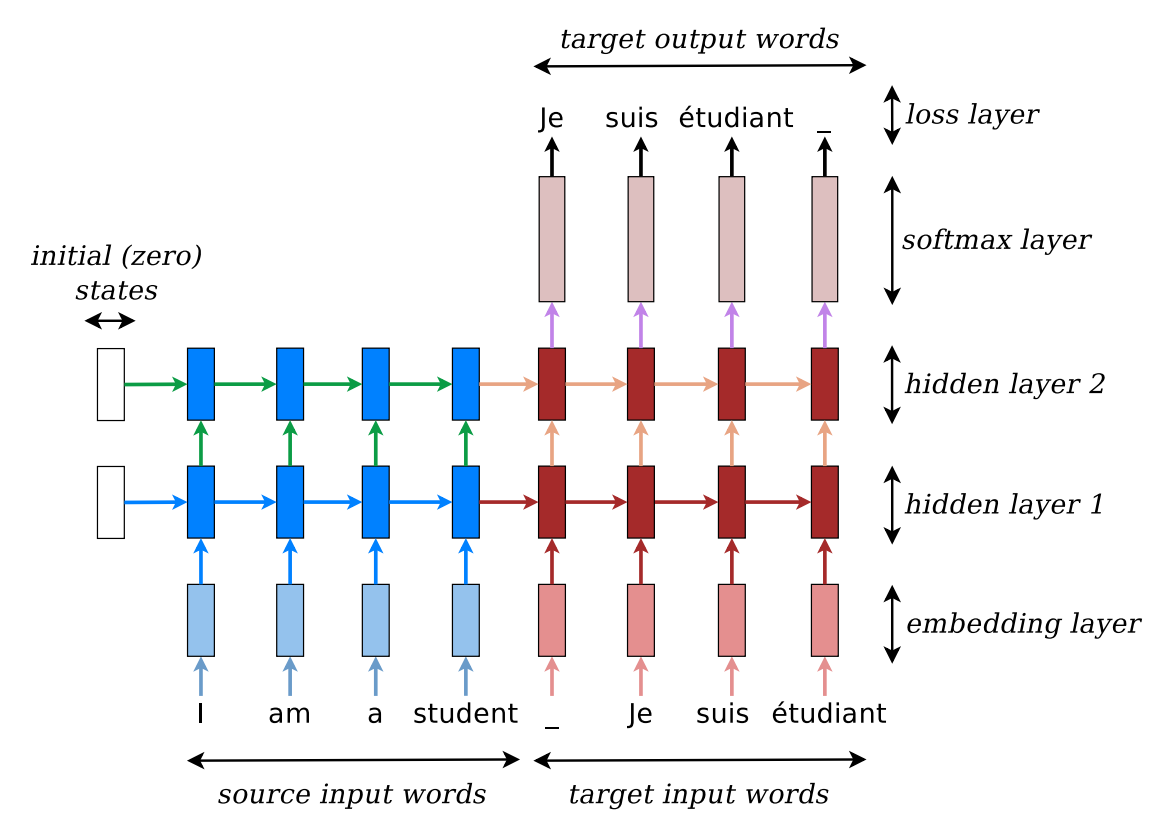
\includegraphics[width=12cm]{nmt}
		\centering
	\end{figure}
	
	Forget gate
	${f_t = \sigma(W_f\cdot[h_{t-1}, x_t] + b_f)}$\\
	
	${i_t = \sigma(W_i \cdot [h_{t-1}, x_t] + b_i)}$\\
	${\tilde{C_t} = tanh(W_C\cdot [h_{t-1}, x_t] + b_C)}$\\
	${C_t =  f_t * C_{t-1} + i_t * \tilde{C_t}}$
	
	Update gate\\
	$z_t = \sigma (W_z x_t + U_z h_{t-1} )$
	
	Drawbacks of the such seq2seq model:
	\begin{enumerate}
	\item The model compresses all information from the input sentence into a hidden vector ${1}$, while ignores the length of input sentence, when the length of input sentence get very long, even longer than the training sentences, it becomes harder to extract specific information for predicting the target word, the performance will get worse.
	\item It's not suitable to assign the same weight to all input words, one target word corresponds usually to one or several words in the input sentence. Treating all words equally does not distinguish the source information and influence the performance badly.
	\end{enumerate}
	
	\subsubsection{Attention Mechanism}
	To solve the problem mentioned above, attention mechanism was proposed to derive a context vector ${c_t}$ that capture the input information to help to predict the target word at time ${t}$. The basic idea is: given the target hidden state ${h_t}$ and the source-side context vector ${c_t}$, we can compute the hidden state ${\tilde{h_t}}$ by combining the current hidden state ${h_t}$ and the context vector ${c_t}$:
		\[ \tilde{h_t} = tanh(W_c[c_t; h_t])\]
	
	Then the target word can be predicted by softmax function:
	\[ p(y_t| y_{\le t, x}) = softmax(W_s \tilde{h_t})\] 

	\begin{figure}[t]
		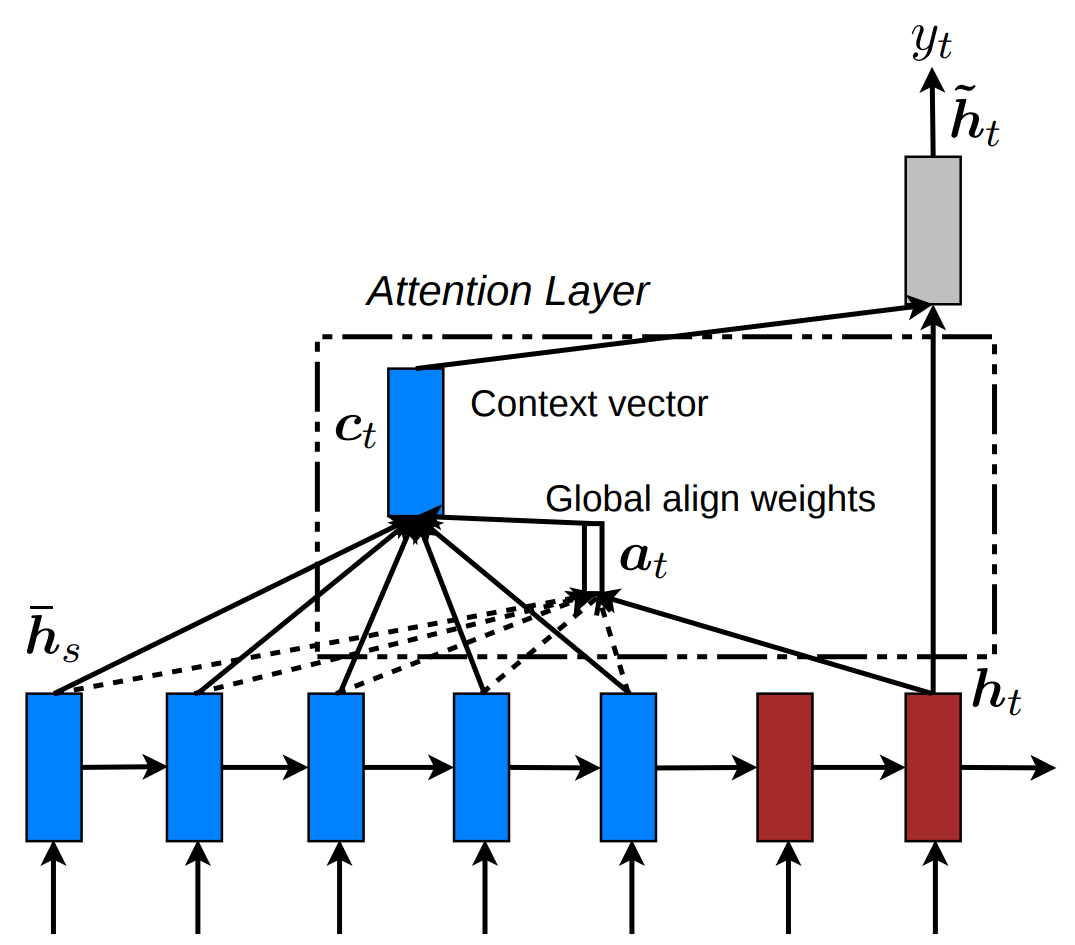
\includegraphics[width=12cm]{attentiong}
		\centering
	\end{figure}
	The concept of attention mechanism comes first from the computer vision domain \cite{xu2015show}, when generating image captions,  The model learns to restrict attention to particular objects in the image.
	
	\cite{bahdanau2014neural}
	Global attention \\
	The global attention attend all the input words, weighted sum of 
	\begin{align}
	a_t(s) = & \ \text{align}(h_t, \bar{h}_s) \\
		   = & \ \frac{\text{exp}(\text{score}(h_t, \bar{h}_s))}{\sum_{s^{\prime}} \text{exp}(\text{score}(h_t, \bar{h}_s^{\prime}))}
	\end{align}
	
	\begin{equation}
	\text{score}(h_t, \bar{h}_s)=\left\{
	\begin{array}{lcl}
	{h_t}^T \bar{h}_s & & dot\\
	{h_t}^T W_a \bar{h}_s & & general\\
	{v_a}^T tanh(W_a[h_t; \bar{h}_s]) & & concat
	\end{array} \right.
	\end{equation}
	
	 with soft attention you need to calculate the attention over all features, however with hard attention, it is a deterministic methods so that 
	Hard attention \\
	Soft attention means when computing the distribution of the alignment, for each word in the input sentence, the model will give a probability.
	
	In comparison with the soft attention, the hard attention will determine a specific word from the input sentence as the alignment and force the alignment probability as ${0}$.  Hard attention mechanism works in image processing however it performs worse in text processing. Because such one-to-one alignment will produce bad translation once a mis-alignment occurs. \cite{luong2015effective} 

	
	Local attention \\
	Since for global attention, for each target word we need to attend the whole input sentence, it is very expensive and impractical to translate longer sentences. Proposed the local attention, the local attention is actually the  tradeoff between soft and hard attention, Soft attention tries to place attention over the whole image "softly" while select one patch of the image to attend. The hard attention need more complicated techniques like variance reduction or reinforcement learning though need less computation when inference.
	
	Local attention: the model first generate an aligned position ${p_t}$ for word at the time ${t}$. Then the context vector ${c_t}$ is a weighted sum within the window ${[p_t-D, p_t+D]}$, ${D}$ is selected empirically. The model predict the aligned  position ${p_t}$ as followed:
	\[ p_t = S \cdot \text{sigmoid}(v_p^T \text{tanh}(W_ph_t))\]
	
	${W_p}$ and ${v_p}$ are the model parameters which will be learned to predict positions.
	To favor the words near position ${p_t}$, we place a Gaussian distribution which centered at ${p_t}$.
	\[a_t(s) = \text{align}(h_t, \bar{h}_s)\text{exp}\Big(-\frac{(s-p_t)^2}{2 \sigma^2}\Big) \]

	\subsubsection{Transformer}
		\begin{figure}[t]
		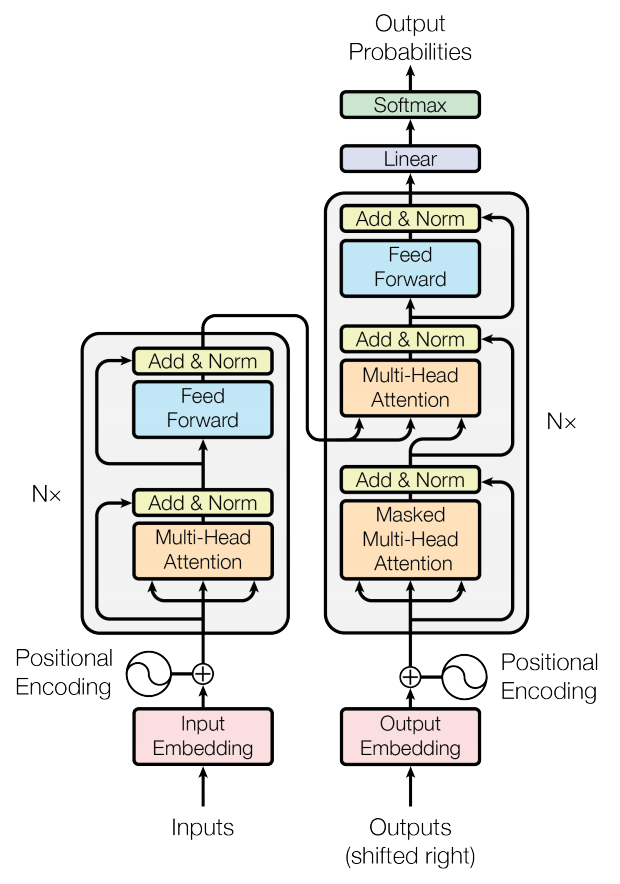
\includegraphics[width=10cm]{transformer}
		\centering
	\end{figure}
	As the illustration above, the long-short term memory (LSTM) and gated recurrent units (GRU) have achieved state of the art in sequence modling and machine translation problem. However the RNN models also have some disadvantages, because of its sequential nature, it is more difficult to fully take advantage of the modern computing devices uch GPU and TPU, which excel at parallel computation not sequential processing.
	
	
	Dot-Product Attention
	a query q and a set of key-value (k-v) pairs to an output, the weight of the each value is the inner product of the query and corresponding key.
	Queries and keys are of the same dimension ${d_k}$, values are of dimension ${d_v}$, than the attention of query on all (k-v) pairs are:
	
	\[ A(q, K, V) = \sum_{i}{ \frac{e^{q\cdot k_i}}{\sum_{j} e^{q\cdot k_j} v_i}}\]
	When we stack the queries ${q}$ to ${Q}$:
	\[ A(Q, K, V) = softmax(QK^T)V\]
	
	As ${d_k}$ get larger, the variance of ${q^T k}$ get larger.  The softmax become very peaked and the gradient get smaller. To counteract this effect, we scaled the dot products by ${\frac{1}{\sqrt{d_k}}}$.
	
	\[ Attention(Q,K,V) = softmax(\frac{QK^T}{\sqrt{d_k}})V\]
	
	
	multi-head attention: first map $Q$,$K$,$V$ into $h$ many lower dimension spaces via linear mapping matrix. Then apply attention and concatenate the outputs. 
	Suppose the original dimensions of queries, keys, values are ${d_model}$. We the number of heads is ${h}$, then ${d_k = d_v = d_{model}/h}$. With ${i \in 1 \cdots h}$ different matrix ${W_i^Q \in R^{d_{model}\times d_k}}$ ${W_i^K \in R^{d_{model}\times d_k}}$ ${W_i^V \in R^{d_{model}\times d_k}}$ and ${W^O \in R^{d_{model}\times d_k}}$.
	
	\[ MultiHead(Q, K, V) = Concat(head_1, \cdots, head_h)W^O \]
	\[head_i = Attention(QW_i^Q, KW_i^K, VW_i^V) \]
	
	
	Transformer reduce the training complexity to a constant ${O(1)}$ number of operations.
	
	
	
	The encoder-decoder attention: the queries come from the previous decoder layer, the keys and values are just the output of decoder. This works as the attention mechanism in the seq2seq model, it allow the decoder to align all positions in the input sequence with different weights
	
	encoder self-attention: all queries, keys, values come from the encoder layer, each position allows to attend to all positions before that position.
	
	decoder self-attention: similar to encoder attention, each position is allowed to attend to position before and including that position.
	
	
	Positional Encoding
	Since there is no RNN or CNN structures in transformer model, we need also need to make use of sequence information for seq2seq learning. We need inject position information into the embedding.
	\[PE_{(pos, 2i)} = sin(pos/ 10000 ^{2i / d_{model}})\]
	\[ PE_{(pos, 2i+1)} = cos(pos / 10000^{2i/d_{model}})\]
	
	
	where pos is the position and $i$ is the dimension. That is, each dimension of 
	
	
	
	
	
	
	
	
	
	
	
	
	
	
	
	
	
	
	
	
	
	
	
	
	
	
	
	
	
	
	
	
	
	